\chapter{Metodologia}

Descrever a metodologia dos testes, como variou o tamanho dos arquivos, quantos arquivos foram utilizados, descrição do computador em que foram feitos os testes.

\section{Resultados}

Analisar os tamanhos dos arquivos compactados a partir dos experimentos realizados. Utilizar tabelas e gráficos para ilustrar o desempenho da sua implementação.

Exemplo de utilização de tabelas.  A Tabela ~\ref{tab:cronograma-1} apresenta um cronograma de execução de um PG fictício.


\begin{table}[htb]
	\centering
	\caption{Cronograma de Atividades do primeiro semestre.}
	\label{tab:cronograma-1}
	\resizebox{\columnwidth}{!}{
		\begin{tabular}{c|c|c|c|c|c|c}
			Atividade & Janeiro/99 & Fevereiro/99  & Março/99  & Abril/99 & Maio/99 & Junho/99\\ \hline
			1&     X      &  	  X   	       &  	X	  	   & 		X	&     X   &      X    \\ \hline
			2&            &  	   	     	   &  	  X  	   & 		X	&         &           \\ \hline
			3&            &  		           &  	  X 	   & 		X   &   X     &     X      \\ \hline
			4&            &  			       &  			   & 	        &         &     X      \\ \hline
			5&            &  			       &  			   & 	        &    X    &   X       \\ \hline
			6&            &  			       &  			   & 	        &         &           \\ \hline
			7&            &  			       &  			   & 	        &         &           \\ \hline
		\end{tabular}
	}
\end{table}


A Figura \ref{fig:graf} exemplifica o uso de uma figura gráfica no texto.


   \begin{figure}[!htb]
    \centering
   	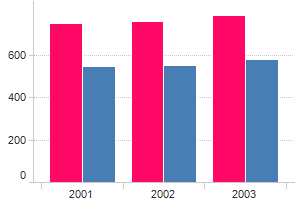
\includegraphics[scale=0.90]{figuras/graf-exemplo.png}
   	\caption{Exemplo de inserção de figura}
   	\label{fig:graf}
   \end{figure}
